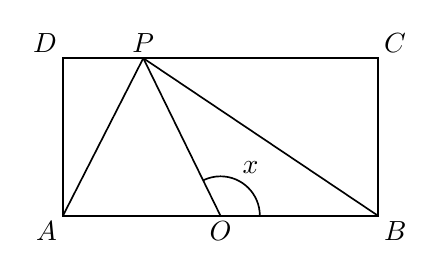
\begin{tikzpicture}[x=1cm,y=1cm,font=\normalsize,
 geometry edge/.style={solid,line width=.6pt},
 geometry mark/.style={solid,line width=.6pt},
 geometry label/.style={font=\normalsize,inner sep=2pt}]
\coordinate (A) at (0,0);
\coordinate (B) at (4,0);
\coordinate (C) at (4,2);
\coordinate (D) at (0,2);
\coordinate (O) at (2,0);
\coordinate (P) at (1.02,2);
\draw[geometry edge] (A)--(B)--(C)--(D)--cycle;
\draw[geometry edge] (A)--(P);
\draw[geometry edge] (P)--(O);
\draw[geometry edge] (P)--(B);
\draw[geometry mark] (O) ++(0:5mm) arc[start angle=0,end angle=116.104854009099,radius=5mm];
\node[inner sep=0pt] at (2.380983001953,0.610943493478) {$x$};
\node[geometry label,below left] at (A) {$A$};
\node[geometry label,below right] at (B) {$B$};
\node[geometry label,above right] at (C) {$C$};
\node[geometry label,above left] at (D) {$D$};
\node[geometry label,below] at (O) {$O$};
\node[geometry label,above] at (P) {$P$};
\end{tikzpicture}
